\documentclass{ximera}

\graphicspath{{./graphics/}{./content/03_15_tangent_planes/graphics/}}

\title{Implicit Curves and Surfaces}
\author{Melissa Lynn}
\outcome{Understand the relationship between the gradient and level curves and surfaces. Use this relationship to find equations for tangent planes.}

\begin{document}
\begin{abstract}
\end{abstract}
\maketitle

By studying directional derivatives and their relationship to the gradient, we observed that the gradient of a function is always perpendicular to its level curves.  That is, we proved the following theorem.

\begin{theorem}
Consider a function $f:\mathbb{R}^n\rightarrow\mathbb{R}$, and suppose $f$ is of class $\mathcal{C}^1$. For some constant $c$, consider the level set
\[
S = \{\vec{x}\in\mathbb{R}^n\;:\;f(\vec{x})=c\}.
\]
Then, for any point $\vec{x}_0$ in $S$, the gradient $\nabla f(\vec{x}_0)$ is perpendicular to $S$.
\end{theorem}

Now, suppose we have a curve defined implicitly. For example, the \emph{Folium of Descartes} is the curve defined by the equation
\[
x^3+y^3=3xy.
\]

\begin{image}
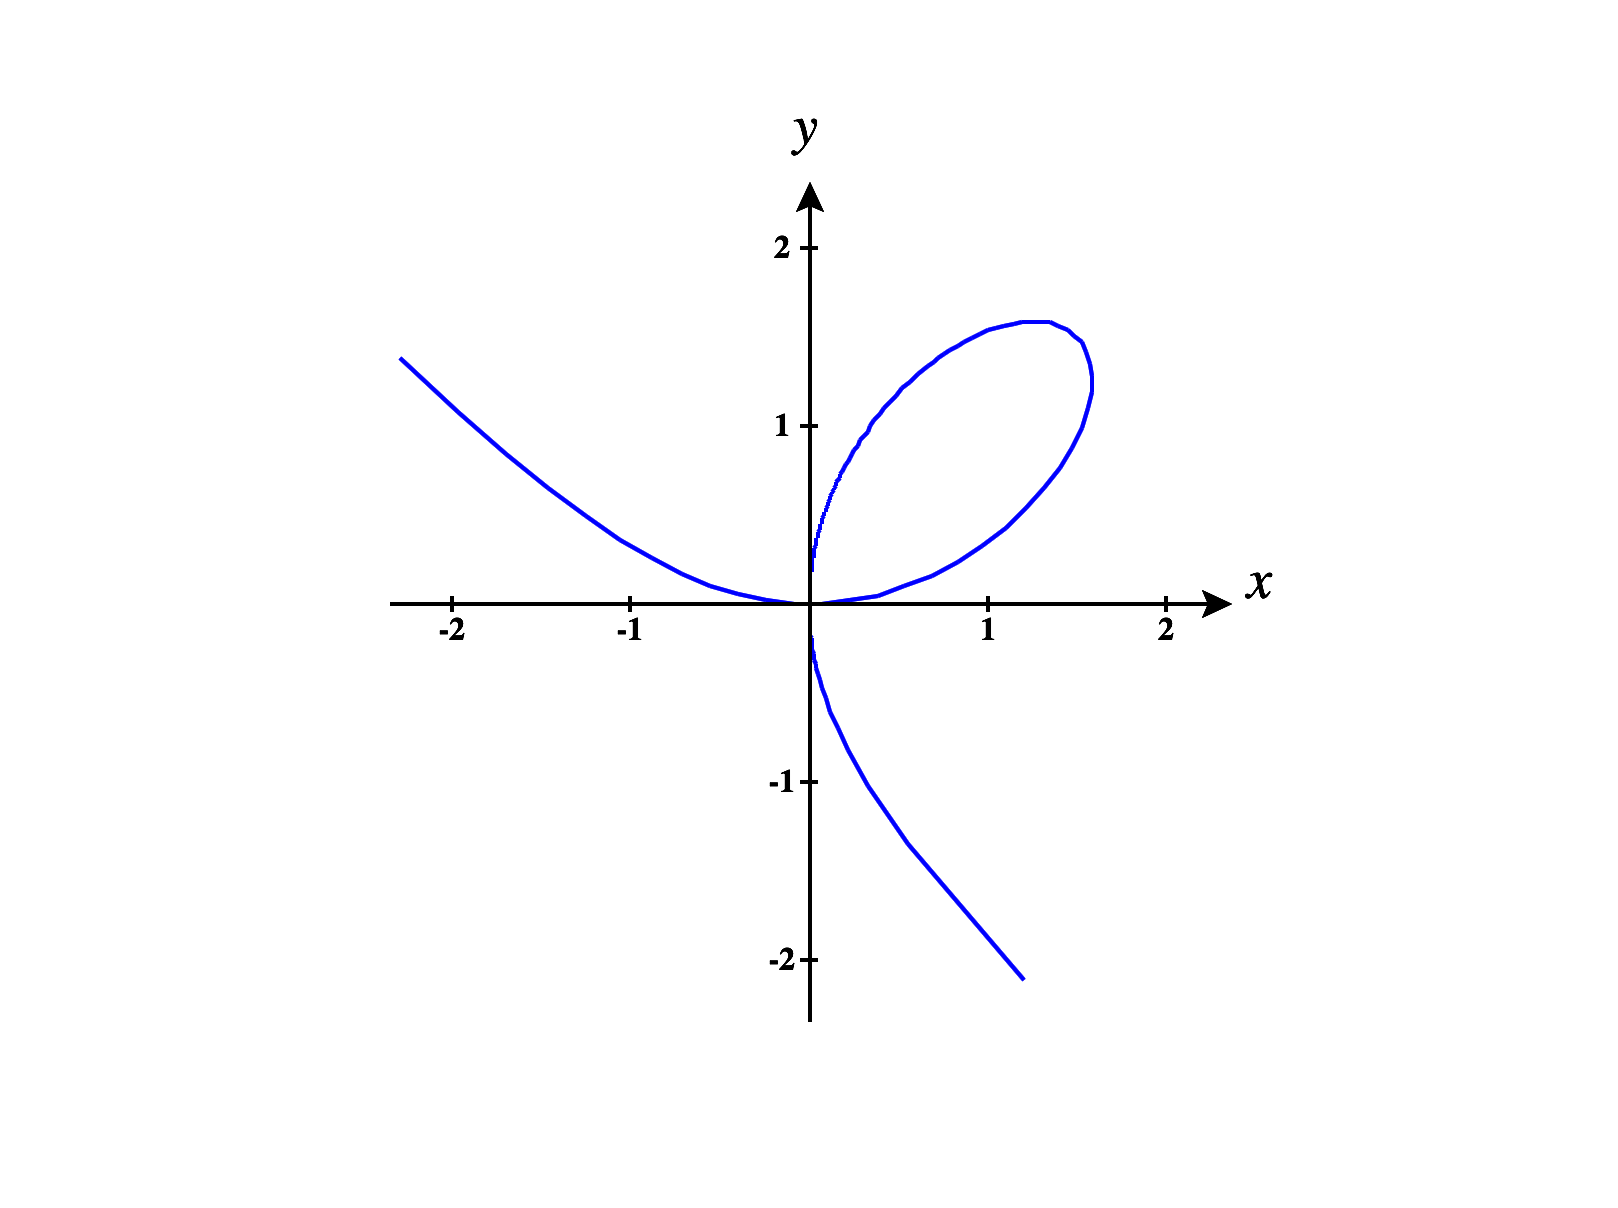
\includegraphics[width = \textwidth]{CalcPlot3D-folium}
\end{image}

Suppose we wanted to find an equation for the tangent line to this curve at the point $\left(\frac{2}{3}, \frac{4}{3}\right)$. Using our knowledge from single variable calculus, there are a couple ways we could approach this problem. We could try to solve for $y$ in terms of $x$, and use the standard single variable methods to find an equation for the tangent line. We could also use implicit differentiation, and find an equation for the tangent line that way.

We will now introduce a new method for finding an equation for the tangent line to this curve, that will use our above observations about the gradient of a function and level sets.

\section*{Tangent lines}

\begin{example}
Consider the Folium of Descartes, $C$, defined by $x^3+y^3=3xy$. We will find an equation for the tangent line to this curve at the point $\left(\frac{2}{3}, \frac{4}{3}\right)$.

\begin{image}
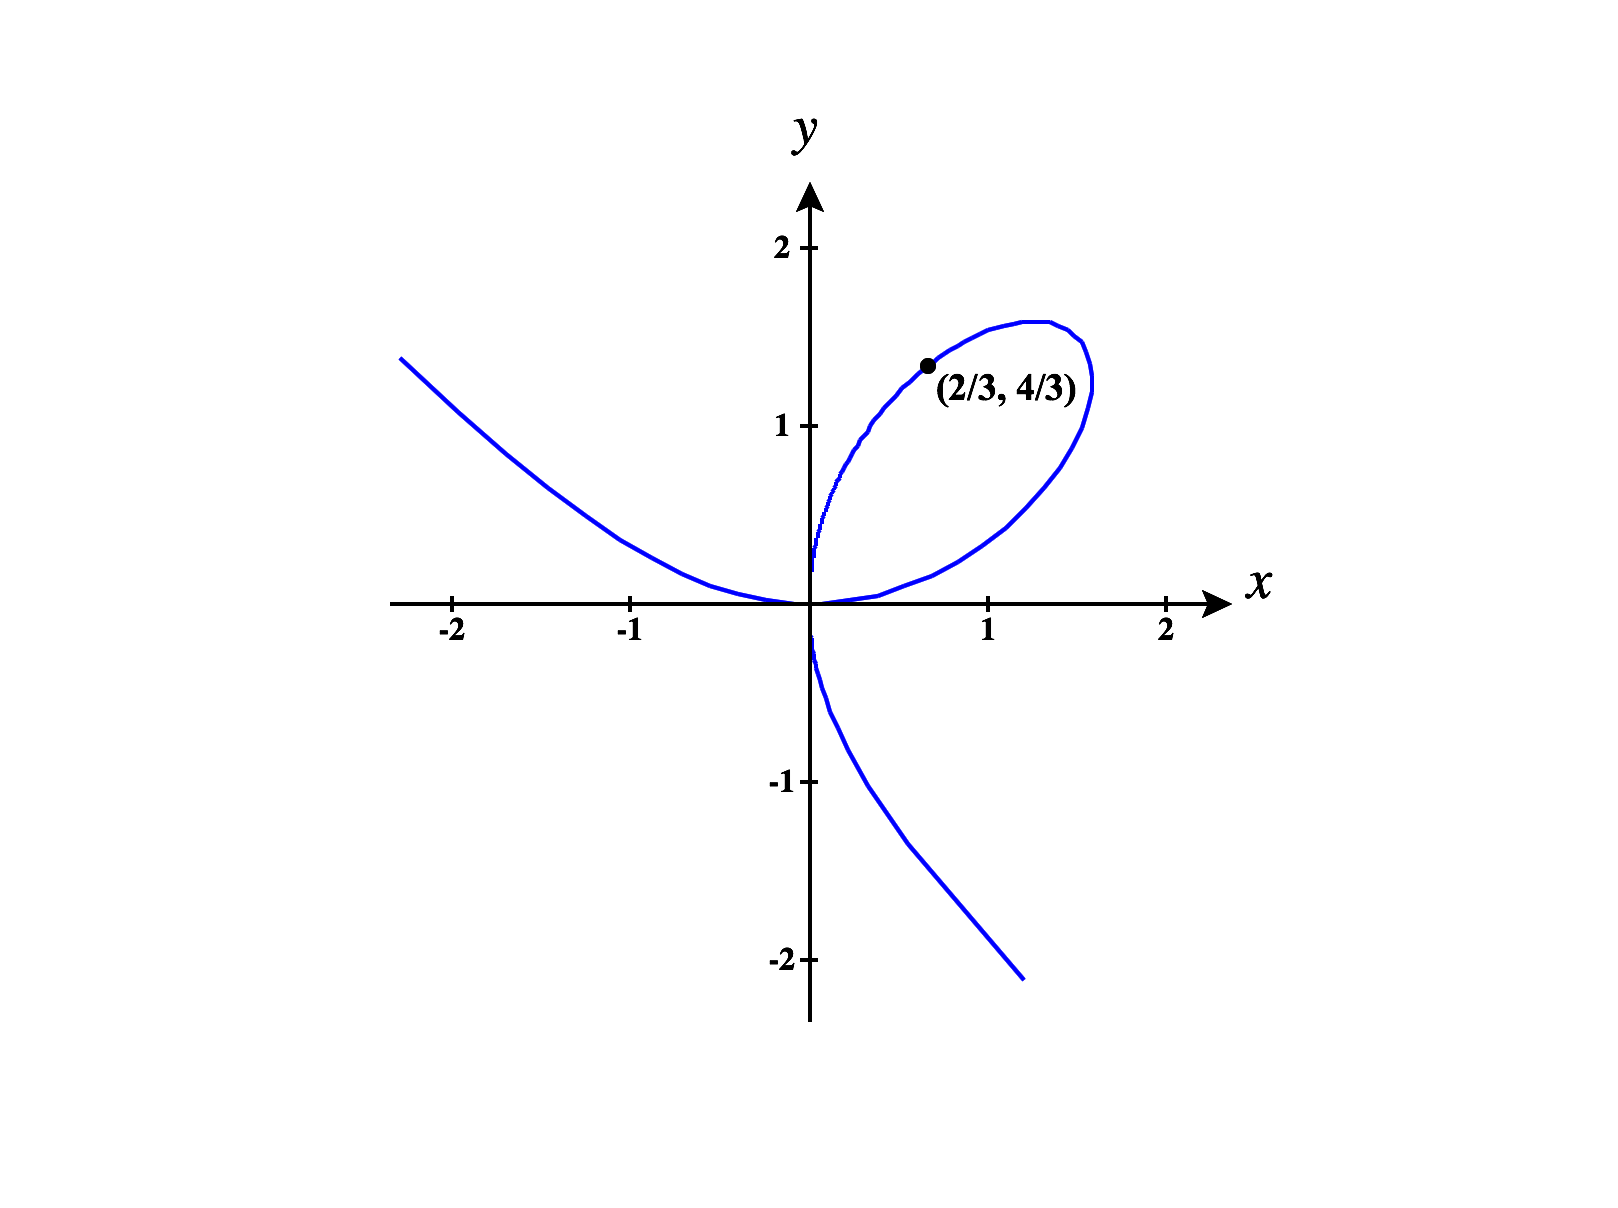
\includegraphics[width = \textwidth]{CalcPlot3D-folium_point}
\end{image}

If we define a function $f(x,y) = x^3+y^3-3xy$, then the curve $C$ is a level set of $f$. In particular, it's the level set $f(x,y)=0$. Then the gradient of $f$ will always be perpendicular to $C$. This means that the tangent line to $C$ at the point $\left(\frac{2}{3}, \frac{4}{3}\right)$ will be perpendicular to $\nabla f\left(\frac{2}{3}, \frac{4}{3}\right)$. In order to take advantage of this fact, we'll compute the gradient of $f$.
\[
\nabla f(x,y) = (3x^2-3y,3y^2-3x)
\]
At the point $\left(\frac{2}{3}, \frac{4}{3}\right)$,
\[
\nabla f\left(\frac{2}{3}, \frac{4}{3}\right) = \left(-\frac{8}{3},\frac{10}{3}\right).
\]
Suppose we have a point $\vec{x} = (x,y)$ on the tangent line. Since $\vec{a} = \left(\frac{2}{3}, \frac{4}{3}\right)$ is also on the tangent line, the vector between these points, $\vec{x}-\vec{a}$, will be contained in the tangent line. That is, it will be parallel to the tangent line.

\begin{image}
\begin{tikzpicture}
\fill (0,0) circle (1pt);
\draw[color = gray] (3.33, -2) -- (-4.67, 8);
\draw[very thick, ->, color = blue] (0,0) -- (.67, 1.33);
\node[anchor = west] at (.67, 1.33) {\color{blue} $\vec{a}$};
\draw[very thick, ->, color = green] (0,0) -- (-2, 4.67);
\node[anchor = east] at (-1, 2.33) {\color{green} $\vec{x}$};
\draw[very thick, ->, color = purple] (.67, 1.33) -- (-2, 4.67);
\node[anchor = west] at (-.67, 3) {\color{purple} $\vec{x} - \vec{a}$};
\draw[color = gray] (3.33, -2) -- (-4.67, 8);
\fill (0,0) circle (1pt);
\end{tikzpicture}
\end{image}

Thus, $\vec{x}-\vec{a}$ must be perpendicular to $\nabla f\left(\frac{2}{3}, \frac{4}{3}\right)$. That is, we must have
\[
\nabla f\left(\frac{2}{3}, \frac{4}{3}\right)\cdot (\vec{x}-\vec{a}) = 0,
\]
which we can rewrite as
\[
\left(-\frac{8}{3},\frac{10}{3}\right) \cdot \left(x - \frac{2}{3}, y-\frac{4}{3}\right)=0.
\]
Expanding the dot product, we obtain the equation,
\[
-\frac{8}{3}\left(x-\frac{2}{3}\right)+\frac{10}{3}\left(y-\frac{4}{3}\right)=0,
\]
which is an equation for the tangent line to $C$ at the point $\left(\frac{2}{3}, \frac{4}{3}\right)$.
\end{example}

\section*{Tangent planes}

We can use a similar method to find equation for tangent planes to surfaces.

\begin{example}
We'll find the tangent plane to the surface $S$ defined by the equation $z^2 +yz = x^2+xy$ in $\mathbb{R}^3$, at the point $(1,1,1)$.

Notice that we can think of $S$ as a level set of the function 
\[
f(x,y,z) = z^2+yz-x^2-xy.
\]
In particular, $S$ is the level set $f(x,y,z) = \answer{0}$.

Knowing that the tangent plane will be perpendicular to the gradient of $f$, we compute
\[
\nabla f(x,y,z) = \answer{(-2x-y,z-x,2z+y)}.
\]
At the point $(1,1,1)$, 
\[
\nabla f(1,1,1) = \answer{(-3, 0, 3)}.
\]

So, the tangent plane will be the plane perpendicular to $(-3,0,3)$, which passes through the point $(1,1,1)$. This plane is defined by the equation
\[
(-3,0,3)\cdot (x-1, y-1, z-1) = 0,
\]
Which can be expanded to
\[
-3(x-1)+3(z-1) = 0.
\]
\end{example}

\end{document}